\section{Data Aggregation}\label{aggregator}
As mentioned in Section~\ref{github}, I decided to use Github as my primary data source and to utilize their \emph{Github APIv3} for this purpose.
The Aggregator and analysis program written for this thesis is named \emph{Gitalizer}.
In this section I will explain the technologies and methods used in the data aggregation process, the database structure and the interaction with Github's \ac{api}.
In the end some problems which occurred during the data collection will be shown as well.


\subsection{Database}\label{data-structure}
To store the gathered Information I chose a \ac{sql} based solution.
PostgreSQL provides excellent tools to ensure a high consistency in your database, namely check constraints, as well as great support for working with times, time zones and locations.
The \ac{sql} database is used in combination with the \ac{orm} library \emph{SQLAlchemy}.


\subsubsection{Database Design}\label{database-design}
The basic schema created for the purpose of this thesis consists of five \ac{orm} models.
A model for Commits, Emails and Repositorys, Contributers as well as Organizations has been created.
The latter is only important to validate results and is not actually used for knowledge discovery, as this is Github specific data.

\begin{figure}[H]
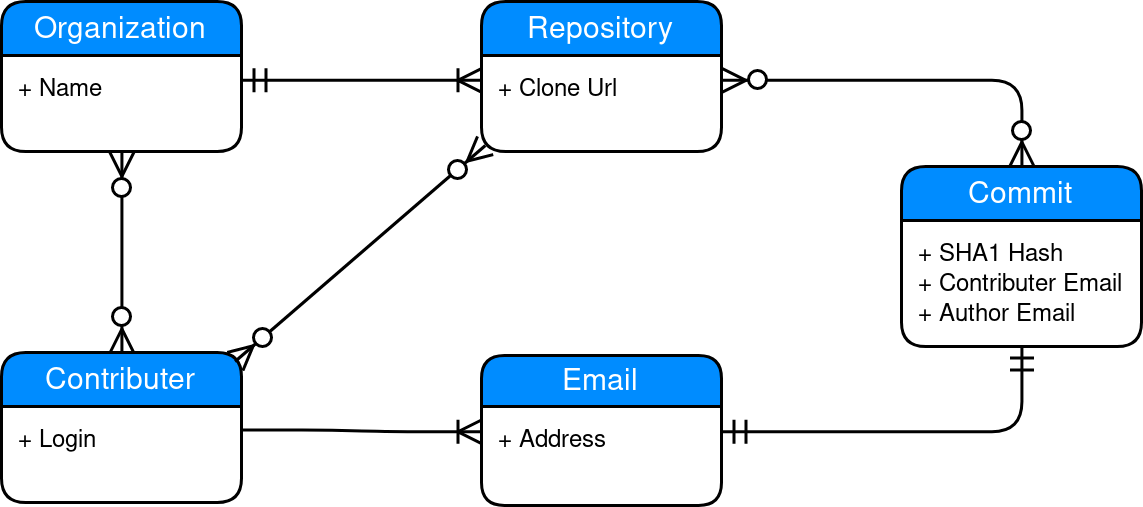
\includegraphics[scale=0.3]{./graphs/gitalizer-data-structure}
\centering
\caption{Gitalizer database relationships.}\label{fig:gitalizer-relationship}
\end{figure}

Every commit of each repository is saved in the database along with its \ac{sha1} hash and the two email addresses as in listing~\ref{lst:raw-commit}.
It is important to note that there is a many-to-many relationship in figure~\ref{fig:gitalizer-relationship} between commits and repositories.
This feature prevents duplication of the same commits from forked repositories.
It is for instance a common practice to create a fork of a repository to develop without intervening with the main git repository of the project.
As described in Section~\ref{internal representation} the probability of a \ac{sha1} collision is highly improbable.
By exploiting this feature it is possible to enforce a unique constraint on the commit hash column, assuming that any duplicated commit hash actually results from a forked or copied repository.
Without this mechanism it could be possible that the same commit of a contributer could be used multiple times as a result of repository forking.
After collecting 43 million commits from Github and actively ignoring obvious project forks, there are still 49 million references between commits and repositories.
This means that about 13\% of gathered commits result from forked repositories which can not easily be identified as such.

As stated above each commit is also saved with its respective email addresses.
There exists a one-to-many relationship between contributers and emails, as every contributer can obtain an unlimited amount of email addresses.
To unambiguously assign a commit to a person, it is necessary to connect all email addresses of these commits to this person.
This relationship does not have a \inlinecode{NOT NULL} constraint as it happens quite often that an email address can not be assigned to any person.
Looking at the collected data it appears that roughly 20\% of collected email addresses from Github are no longer connected to an active user.

As stated in Section~\ref{github-organization} Github provides a way to organize several people in organizations and teams.
As one of the goals of this thesis is to see if it is possible to detect member of an organization in open-source projects, a model for organization has been created as well.
This data can then be used to check against the results of this research's results.


\subsection{Gitalizer}
The Program written for this thesis features data aggregation, preprocessing, knowledge extraction and visualization.
Gitalizer uses a PostgreSQL database for data storage and data consistency checks as described in~\ref{data-structure}.
For interaction with the Github \ac{api} the \emph{PyGithub} library is used, which provides a convenient abstraction layer for requests and automatically maps \ac{json} responses to \emph{Python} objects.

The data aggregation module of Gitalizer is capable of several approaches for gathering data.
In the following we will look at those approaches in detail.

\begin{description}
    \item[Git repository]\label{stand-alone-repository-scan} \hfill \\
        Gitalizer can scan any git repository from a \ac{ssh} or \ac{http} \acs{url} as long as the current user has access to it.
        The repository is cloned into a local directory and when the cloning finished the actual scanning process begins.
        During the scan, we git checkout the \emph{HEAD} of the current default branch for this repository and walk down every reachable commit of the Git history.
        The program saves all available meta data for each commit in its database, namely the emails, timestamps and names of the committer as well as additions and deletions to the project in lines of code.

        After this scan we are still missing a lot of information.
        The unique identifier of an author or committer is their email address, as names may change or can be ambiguous.
        The problem with the simplicity of Git is that there exists no concept of an user.
        Thereby we cannot easily link email addresses to a specific contributer without additional metadata.


    \item[Github Repository]\label{github-repo-scan} \hfill \\
        To tackle the problem of missing meta data in~\ref{stand-alone-repository-scan}, I used the Github \ac{api} to get some of the missing meta data.
        The general approach is the same as in the previous scan method. The repository is cloned and locally scanned.
        However, a request to Github is issued every time a email is found, which we do not already have linked to a contributer.
        Github allows to link multiple email addresses with a single user account and automatically references the respective user in their own \ac{api} commit representation.
        With this additional meta data we gain ground truth about the identity of an author or committer.

        Anyway this approach does not work, if the user of a commit removes the email, which has been used for the commit, from his account or if the user deletes their account.
        If this happens and the email contributor relationship has not already been created, there is nothing that can be done and these commits need to be handled later on in the preprocessing of the data.

    \item[Github User]\label{github-repo-scan} \hfill \\
        To try getting all repositories of a specific user a new functionality, which highly utilizes the Github \ac{api}, has been added.
        At first several requests are issued to get all repositories of the specified user, as well as all starred repositories of this user.
        During the repository exploration, every relevant repository is added to a shared queue, lets call it ``repo-queue'', which is then processed by a multiprocessing pool of workers.
        Each worker process then scans a single repository as described in~\ref{github-repo-scan} and gathers missing meta data as described in~\ref{github-repo-scan}.


    \item[Connected users]\label{github-repo-scan} \hfill \\
        For detection and analysis of connections between contributers over multiple repositories additional user repository discovery as described in~\ref{requirements}, another feature has been added to Gitalizer.
        Gitalizer is able to achieve this by not just scanning a single user, but rather scanning the repositories of the specific user, as well as the repositories of all following and followed users as described in~\ref{github-user-scan}.
        For this task two different worker pools are utilized.
        The user discovery pool is initialized with a shared queue, lets call it ``user-queue'', of all users we need to look at.
        This pool simply searches for relevant repositories of each user and passes the repository \ac{url} to a second shared queue.
        The second pool then processes the ``repo-queue'' as described in~\ref{github-repo-scan}.

        For organizations it's nearly the same approach.
        Initially all repositories, which are owned by the organization, are added to the ``repo-queue''.
        All publicly visible organization members are then added to the ``user-queue'' and processed as described above.
\end{description}


\subsection{Database optimization}
As the database kept growing, several adjustments in the database schema and setup had to be made.
After reaching about 12\ac{GB}, the database write and read operations took longer than the actual aggregation process.
The performance of the database has then been continuously increased in several steps.
One of the first counter measures was the reduction of commits in the database using \ac{sha1} as stated in Section~\ref{database-design} and the ignoring of forked repositories to reduce a bloating of the relation table between commits and repositories.
Another performance boost has been achieved by disabling or loosen several fail-safe mechanisms of PostgreSQL, namely `synchronous commit' and `write ahead' parameter, which are designed to save data on a system crash.
As there is no important or critical data handled it was acceptable to pass on these mechanisms.


\subsection{Incremental aggregation}
To ensure a constantly up to date database Gitalizer needed to be capable of fast rescans of repositories.
The initial scan of a repository always includes cloning, scanning the whole repository and writing it into the database.
After a repository is scanned completely at least once it is marked as as such and won't ever by completely scanned again.
All following runs then only clone the repository and scan the newest unknown commits.
These are discovered by performing a breadth first search until no new nodes are found.

As explained in Section~\ref{more-git-features} it is possible to rewrite commits and force push them.
This scenario needs to be explicitly handled since force pushes can completely alter the history of a git repository, which can subsequently lead to a split in the Git history and leaves dangling commits.
As the complete history of a repository is stored inside the database, Gitalizer needs to detect a force push by walking down the git history tree until it finds known commits.
If any of these commits has children, which are not in the newly scanned commits, a force push took place and the old commit history has to be truncated, since it is now outdated and irrelevant.
\todo{Grafik zu dieser git force push}


\subsection{Problems}
During the development of the data aggregator I experienced a few problems and edge cases which needed to be handled.
The earliest and most delaying problem was the rate limit of the Github \ac{api}, which limits to 5000 requests per hour.
But beside this rate limiting there also is an abuse detection mechanism, which triggers, if too many requests are fired in a short amount of time.

The first version of the aggregator didn't clone and scan the repository locally, but rather gathered all information from the Github \ac{api} endpoints.
This approach worked well until the aggregator hit the official repository of Nmap, which has about 11.000 commits and took over three hours to scan.
Soon I realized that this would severely slow down my research and I then started to continuously minimize the amount \ac{api} calls issued by Gitalizer.
A connected user scan of my own Github account led to about 600.000 commits and took about one and a half day on the final working version of Gitalizer, to provide you with a reference of scale.

After implementing multiprocessing, I managed to hit the rate limit again, as I was now issuing requests with many threads.
To fix this issue I implemented a wait and retry wrapper around every single function call or object access, which triggered a call to the Github \ac{api}.
Afterwards the aggregator was capable of running multiple days without worker processes silently dying or incomplete collected data.

Fine tuning the edge cases and the handling of the \ac{api} took about 3 months, since there were many problems such as unpredictable error responses from github, missing data in queries or simply unknown or broken encodings in Github's meta data.

